\documentclass[10pt,a5paper]{extarticle}
\usepackage[margin=1.25cm]{geometry}
\usepackage[utf8]{inputenc}
\usepackage[IL2]{fontenc}
\usepackage[czech]{babel}
\usepackage{microtype}
\usepackage{amssymb}
\usepackage{amsthm}
\usepackage{amsmath}
\usepackage{xcolor}
\usepackage{graphicx}

\usepackage[inline]{enumitem}

\newcommand{\R}{\mathbb{R}}

\setlist[enumerate]{label={(\alph*)},topsep=\smallskipamount,itemsep=\smallskipamount,parsep=0pt,itemjoin={\qquad}}
\setlist[itemize]{topsep=\smallskipamount,noitemsep}

\def\tisk{%
\newbox\shipouthackbox
\pdfpagewidth=2\pdfpagewidth
\let\oldshipout=\shipout
\def\shipout{\afterassignment\zdvojtmp \setbox\shipouthackbox=}%
\def\zdvojtmp{\aftergroup\zdvoj}%
\def\zdvoj{%
    \oldshipout\vbox{\hbox{%
        \copy\shipouthackbox
        \hskip\dimexpr .5\pdfpagewidth-\wd\shipouthackbox\relax
        \box\shipouthackbox
    }}%
}}%

\newtheorem*{poz}{Pozorování}

\theoremstyle{definition}
\newtheorem{uloha}{Úloha}
\newtheorem{suloha}[uloha]{\llap{$\star$ }Úloha}
\newtheorem*{bonus}{Bonus}
\newtheorem*{defn}{Definice}

\pagestyle{empty}

\newcommand{\sitem}{\item[\addtocounter{enumi}{1}{\footnotesize$\star$}(\alph{enumi})]}


\def\st{^\circ}

\let\ee\expandafter

\def\vysld{}
\let\printvysl\relax

\makeatletter
\long\def\vyslplain#1{\ee\ee\ee\gdef\ee\ee\ee\vysld\ee\ee\ee{\ee\vysld\ee\printvysl\ee{\the\c@uloha}{#1}}}

\def\locvysl#1{\ee\gdef\ee\locvysld\ee{\locvysld\item #1}}
\let\lv\locvysl

\newenvironment{ulohav}[1][]{\begin{uloha}[#1]\gdef\locvysld{\begin{enumerate}}}{\ee\vyslplain\ee{\locvysld\end{enumerate}}\end{uloha}}
\newenvironment{sulohav}[1][]{\begin{suloha}[#1]\gdef\locvysld{\begin{enumerate*}}}{\ee\vyslplain\ee{\locvysld\end{enumerate*}}\end{suloha}}

\makeatother

\let\vysl\vyslplain

\begin{document}

%\tisk

\section*{4. Opáčko na čtvrtletku aneb Vesměs vykrádačka Petákové}


\mathcode`\,="013B


\begin{ulohav}
Dopočtěte velikosti všech úhlů a délky všech stran ve standardně značeném trojúhelníku $ABC$, pro který platí
\begin{enumerate}
    \item $a = 10$, $\alpha = 62^\circ$, $\beta = 34^\circ$\lv{$b\doteq6,3$; $c\doteq11,3$; $\gamma=84\st$} % 74a
    \item $b = 6$, $c = 9$, $\beta = 75\st$\lv{neexistuje} % 75b
     \item $b = 8$, $c = 5$, $\gamma = 26\st55'$\lv{(I) $a_1\doteq10,6$, $\beta_1\doteq46\st25'$, $\alpha_1\doteq106\st34'$, (II) $a_2\doteq3,7$, $\beta_2\doteq133\st25'$, $\alpha_2\doteq19\st40'$} % 75c
\end{enumerate}
\end{ulohav}


\begin{ulohav}
V krychli $ABCDEFGH$ (o hraně délky 1) určete
\begin{enumerate}
    \item odchylku přímek $AE$ a $BH$,\lv{$54\st44'$} %29e
    \item odchylku přímky $AS_{EG}$ od roviny $CDH$,\lv{$24\st06'$} %33e
    \sitem vzdálenost bodu $H$ od přímky $AS_{CG}$,\lv{1} %17g
    \item vzdálenost bodu $S_{EF}$ od roviny $ABG$\lv{$\frac{\sqrt2}{2}$} %24e
\end{enumerate}
\end{ulohav}

\begin{ulohav}
V pravidelném čtyřbokém jehlanu, jehož podstavná hrana má délku 4 a výška je 6, určete
\begin{enumerate}
    \item vzdálenost bodu $S_{CV}$ od přímky $AV$\lv{$\frac{6}{11}\sqrt{22}$} %19c
    \item vzdálenost bodu $A$ od roviny $BCV$\lv{$\frac{6}{5}\sqrt{10}$}
    \item odchylku přímek $AC$ a $VS_{BC}$\lv{$77\st05'$} %31g
    \item odchylku rovin $ADV$ a $BCS_{AV}$\lv{$63\st26'$} %36f
\end{enumerate}
\end{ulohav}


\begin{uloha}[Tato úloha bude v následujícím domácím úkolu]
Určete objem rotačního tělesa, které vznikne rotací obdélníkového papíru o rozměrech\footnote{Tento poměr stran, $1 : \sqrt2$, mají všechny papíry řady A (A4, A5 atd.), až na drobné zaokrouhlení.} $1 \times \sqrt2$ kolem jeho diagonály. Uveďte \emph{nezaokrouhlený} výsledek (tj. se zlomky, odmocninami atd.).
\[ 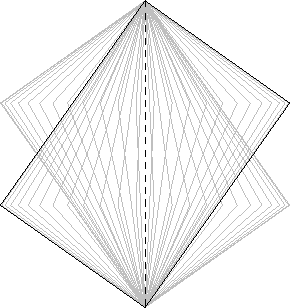
\includegraphics{rotaze_tikz.pdf} \]
\end{uloha}


\newpage
\parindent=0pt
\parskip=\smallskipamount
\def\printvysl#1#2{\textbf{#1.}\ #2\par}
\vysld



\end{document}